\documentclass{beamer}

\usepackage[utf8]{inputenc}
\usepackage{amsmath}
\usepackage{makecell}
\usepackage{bm}
\usepackage[square, numbers, comma, sort&compress]{natbib}
\usepackage{subcaption}

\usetheme{Warsaw}
\setbeamertemplate{bibliography item}{\insertbiblabel}

%Information to be included in the title page:
\title[Hierarchical visualization of scRNA-seq data]{Using probabilistic methods for hierarchical visualization of single-cell RNA-seq data}
\author{Tobias Beers}
\institute{Universiteit van Amsterdam}
\date{July 22nd, 2020}

\logo{
\includegraphics[height=0.75cm]{clslogo.png}}

\begin{document}


% advi en nuts slides


\frame{\titlepage}

\begin{frame}{Layout}
    \tableofcontents
\end{frame}

\section{Introduction}

\subsection{scRNA-seq data and dimensionality reduction}

\begin{frame}{Gene expression and scRNA-seq}
\begin{itemize}
    \item Gene expression: DNA $\rightarrow$ mRNA $\rightarrow$ gene product
    \item High expression of a gene means more mRNA
    \item Single-cell RNA sequencing (scRNA-seq) measures relative gene expression by quantifying mRNA transcripts
    \item ScRNA-seq data may contain thousands of dimensions (genes), but visualization is easier in two dimensions
\end{itemize}
\end{frame}

% \subsection{Dimensionality reduction}

\begin{frame}{Dimensionality reduction}
\begin{columns}
\begin{column}{0.5\textwidth}
    \begin{itemize}
    \item linear techniques
    \begin{itemize}
        \item PCA
        \item PPCA
        \end{itemize}
        \item non-linear techniques
        \begin{itemize}
        \item t-SNE
        \item UMAP
        \item Hierarchical Mixture of PPCAs (HmPPCAs)
        \end{itemize}
    \end{itemize}
\end{column}
\begin{column}{0.5\textwidth}
\begin{figure}
    \centering
    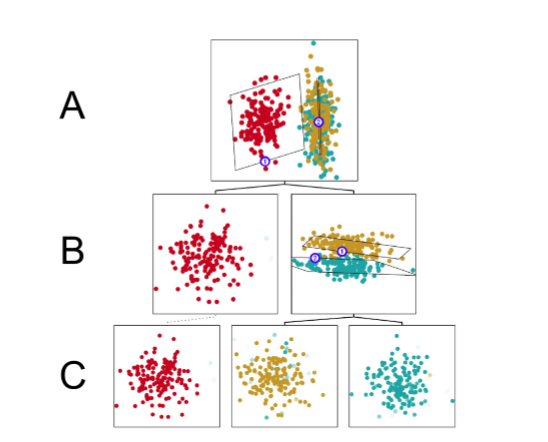
\includegraphics[width=\linewidth]{hierarchy_bishoptipping.png}
    % \caption{Caption}
    % \label{fig:my_label}
\end{figure}
\footnotesize
Figure has been copied from Bishop \& Tipping (1998) \cite{bishop1998hierarchical}
\end{column}
\end{columns}
\end{frame}


\begin{frame}
\frametitle{Innovation and relevance}
\begin{itemize}
    \item HmPPCAs has been used on scRNA-seq data before \cite{philipsthesis}
    \item So far, HmPPCAs tree has been built interactively
    \begin{itemize}
        \item Automatic Clustering
    \end{itemize}
    \item HmPPCAs is solved through expectation-maximization (EM) algorithm
    \begin{itemize}
        \item Probabilistic programming
    \end{itemize}
\end{itemize}
\end{frame}

\subsection{Theory behind probabilistic hierarchical visualization}

\begin{frame}{PPCA}
% \begin{columns}
% \begin{column}{0.5\linewidth}
\begin{itemize}
    \item Full data-set $\bm{X}$, latent data-set $\bm{Z}$
    \item Latent data ($m$ dimensions) is transformed into full data-set ($d$ dimensions): $\bm{x}_i = \bm{W}\bm{z}_i+\bm{\mu}+\bm{\epsilon}$
    \begin{itemize}
        \item $\bm{W}$: factor loadings, $\bm{\mu}$: added means, $\bm{\epsilon}$: noise
    \end{itemize}
    % \item $\bm{\epsilon}$ comes from normal distribution $\mathcal{N}(\epsilon|\bm{0},\sigma^2 \bm{I_d})$
    \item Therefore, $\bm{x}|\bm{z}$ follows the distribution $\mathcal{N}(\bm{x}|\bm{Wz}+\bm{\mu}, \sigma^2\bm{I})$
    % \begin{itemize}
    %     \item $p(\bm{X}|\bm{W}, \bm{\mu}, \sigma) = \prod^n_{i=1} p(\bm{x}_i)p(\bm{z}_i)$
    % \end{itemize}
\end{itemize}

\begin{figure}
    \centering
    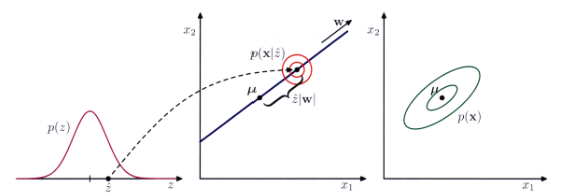
\includegraphics[width=.8\textwidth]{Screenshot_2020-07-14 Pattern Recognition and Machine Learning - Bishop_PatternRecognitionAndMachineLearning pdf.png}
    % \caption{Caption}
    % \label{fig:my_label}
\end{figure}
\footnotesize
Figure has been copied from Bishop (2006) \cite{bishop2006pattern}. $m=1, d=2$
% \end{column}
% \begin{column}{0.5\linewidth}

% \end{column}
% \end{columns}
\end{frame}

\begin{frame}{Mixture of PPCAs (MoPPCAs)}
\begin{itemize}
    \item Suppose our data-set is the result of $K$ latent variable models
    \item Now, $p(\bm{x}_i|\bm{\mu}, \bm{\sigma}^2, \bm{\pi}, \bm{W}) = \sum^K_{k=1}\pi_k \mathcal{N}(\bm{x}|\bm{W}_k\bm{z}_k+\bm{\mu}_k, \sigma^2_k\bm{I})$
    \begin{itemize}
        \item Where the mixture coefficient $\pi_k$ denotes which proportion of the data comes from mixture component $k$
    \end{itemize}
    % \item Responsibility term $\gamma^k_i$ notes the probability that data-point $\bm{x}_i$ comes from mixture component $k$ 
    % \item $\gamma^k_i = \frac{\pi_k p(\bm{x}_i)}{\sum^K_{j=1} \pi_j p(\bm{x}_i)} = \frac{\pi_k \mathcal{N}(\bm{x}_i|\theta_k)}{\sum^K_{j=1} \pi_j \mathcal{N}(\bm{x}_i|\theta_j)}$
    % \item Then log-likelihood becomes $\ln{p(\bm{X}, \bm{Z} | \theta)} = \sum^N_{i=1} \sum^K_{j=1} \gamma^k_i \ln{\pi_k \mathcal{N}(\bm{x}_i|\bm{W}_k\bm{z}_k+\bm{\mu}_k, \sigma^2_k\bm{I}) \mathcal{N}(\bm{z}_i|\bm{0},\bm{I})}$
\end{itemize}

\begin{figure}
    \centering
    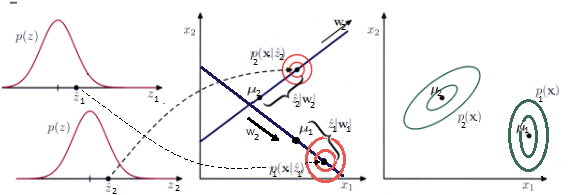
\includegraphics[width=.8\textwidth]{moppcas.png}
    % \caption{Caption}
    % \label{fig:my_label}
\end{figure}
\footnotesize
Figure has been copied and modified from Bishop (2006) \cite{bishop2006pattern}. $m=1, d=2, K=2$
    
\end{frame}

\begin{frame}{Hierarchical Mixture of PPCAs (HmPPCAs)}
    
    \begin{columns}
\begin{column}{0.5\textwidth}
    \begin{itemize}
        \item We can add more levels: suppose mixture component $k$ consists of multiple sub-components $m$
        % \item log-likelihood extends to $\sum^n_{i=1} \sum^K_{k=1} \gamma^k_i \sum_{m=1}^{|\mathcal{G}_i|} \gamma_i^{m|k} \ln{\pi_{m|k} p(\bm{x}_i, \bm{z}_i)}$
        \item As many levels can be added as necessary!
    \end{itemize}
\end{column}
\begin{column}{0.5\textwidth}
\begin{figure}
    \centering
    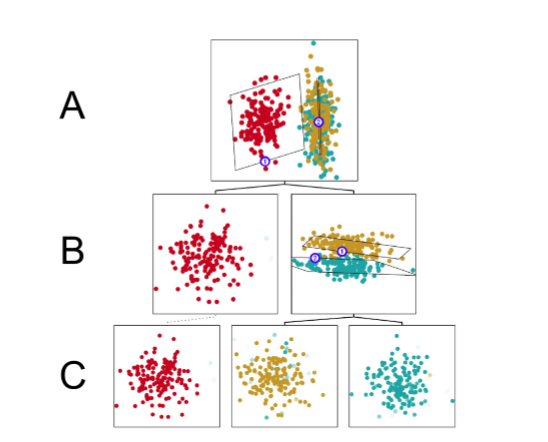
\includegraphics[width=\linewidth]{hierarchy_bishoptipping.png}
    % \caption{Caption}
    % \label{fig:my_label}
\end{figure}
\footnotesize
Figure has been copied from Bishop \& Tipping (1998) \cite{bishop1998hierarchical}
\end{column}
\end{columns}
    
\end{frame}



\subsection{Probabilistic programming: Stan}

\begin{frame}
\frametitle{Stan}
    \begin{columns}
\begin{column}{0.5\textwidth}

    \begin{itemize}
    \item Probabilistic Programming Language
    \item Specify a model, input data and Stan finds posterior distribution of parameters given observed data
    \item Easy add changes to model
    \item Two methods of inference:
    \begin{itemize}
        \item NUTS
        \item ADVI/VB
    \end{itemize}
\end{itemize}

\begin{figure}
    \centering
    
\includegraphics[width=.2\linewidth]{stan_logo.png}
    % \caption{Caption}
    % \label{fig:my_label}
\end{figure}

\end{column}
\begin{column}{0.5\textwidth}
\begin{figure}
    \centering
    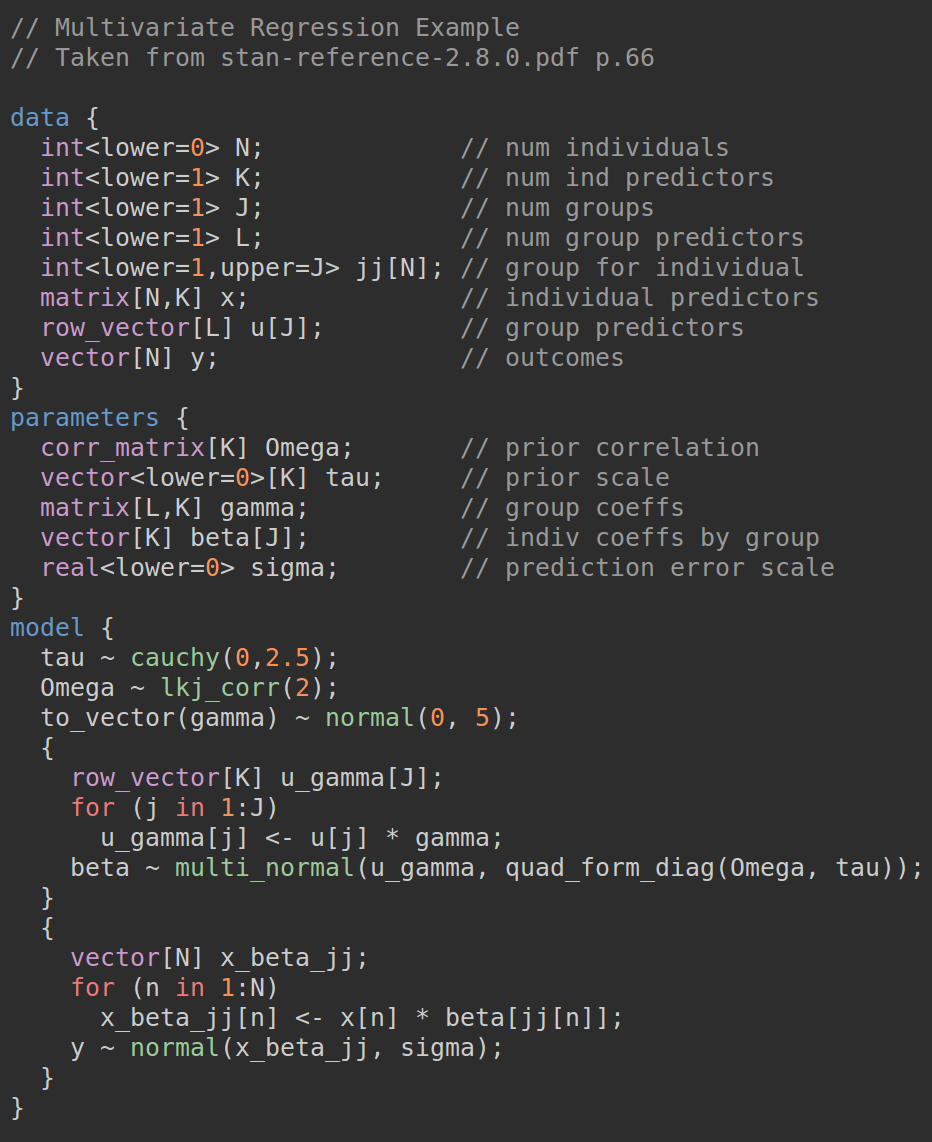
\includegraphics[width=.9\linewidth]{stan_example.png}
    % \caption{Caption}
    % \label{fig:my_label}
\end{figure}
\end{column}
\end{columns}
    

\end{frame}

% \begin{frame}{NUTS}
% \begin{columns}
% \begin{column}{0.5\textwidth}
%     \begin{itemize}
%         \item \textbf{Metropolis-Hastings}
%         \begin{itemize}
%             \item \color<.>{black} Convergence takes long due to inefficient pathways
%         \end{itemize}
%         \color{gray}
%         \item Hamiltonian Monte Carlo
%         \item NUTS
%     \end{itemize}
% \end{column}
% \begin{column}{0.5\textwidth}
% \begin{figure}
%     \centering
%     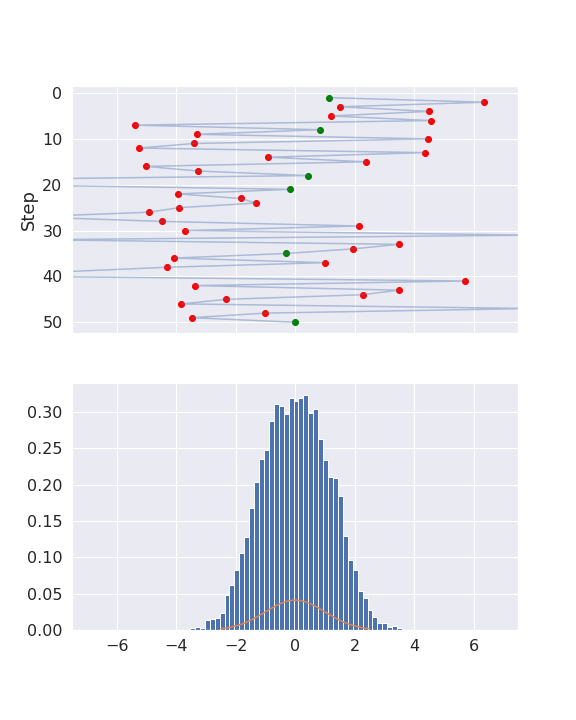
\includegraphics[width=\linewidth]{samplingresult.png}
%     % \caption{Caption}
%     % \label{fig:my_label}
% \end{figure}

% \end{column}
% \end{columns}
% \end{frame}

% \begin{frame}{NUTS}
% \begin{columns}
% \begin{column}{0.5\textwidth}
%     \begin{itemize}
%     \color{gray}
%         % \item Metropolis-Hastings
%         \color{black}
%         \item \textbf{Hamiltonian Monte Carlo}
%         \begin{itemize}
%             \item Faster convergence
%             \item Need to pick values for path-length $L$ and step-size $\epsilon$
%         \end{itemize}
%         \color{gray}
%         \item NUTS
%     \end{itemize}
% \end{column}
% \begin{column}{0.5\textwidth}
% \begin{figure}
%     \centering
%     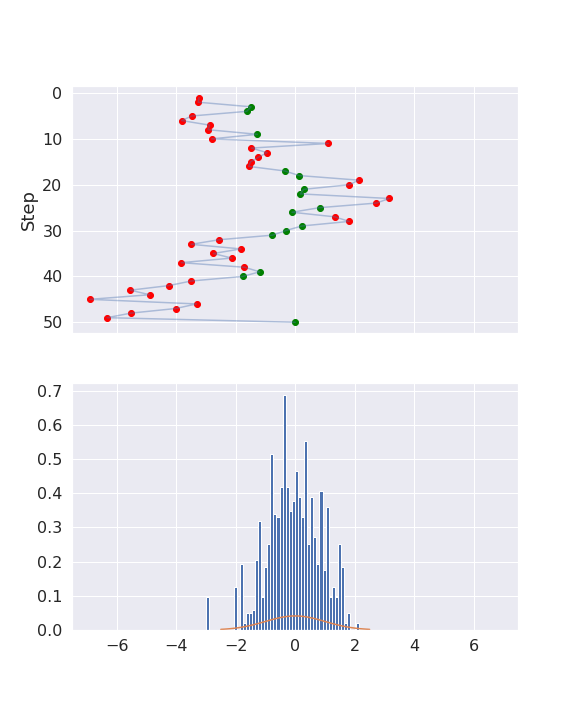
\includegraphics[width=\linewidth]{samplingresult_hmc.png}
%     % \caption{Caption}
%     % \label{fig:my_label}
% \end{figure}

% \end{column}
% \end{columns}
% \end{frame}

% \begin{frame}{NUTS}
%     \begin{itemize}
%     % \color{gray}
%         % \item Metropolis-Hastings
%         \color{black}
%         \item Based on Hamiltonian Monte Carlo
%         \begin{itemize}
%             % \item Faster convergence
%             \item Fictive particle moves through sample space
%             \item New positions are accepted or rejected as sample
%             \item Need to pick values for path-length $L$ and step-size $\epsilon$
%         \end{itemize}
%         \color{gray}
%         \item NUTS
%     \end{itemize}
% \end{frame}


% \begin{frame}{NUTS}
% \begin{columns}
% \begin{column}{0.5\textwidth}
%     \begin{itemize}
%     \color{gray}
%         % \item Metropolis-Hastings
%         \item Hamiltonian Monte Carlo
%         \color{black}
%         \item \textbf{NUTS}
%         \begin{itemize}
%             \item Automatically tunes path-length $L$ and step-size $\epsilon$
%         \end{itemize}
%     \end{itemize}
% \end{column}
% \begin{column}{0.5\textwidth}
% \begin{figure}
%     \centering
%     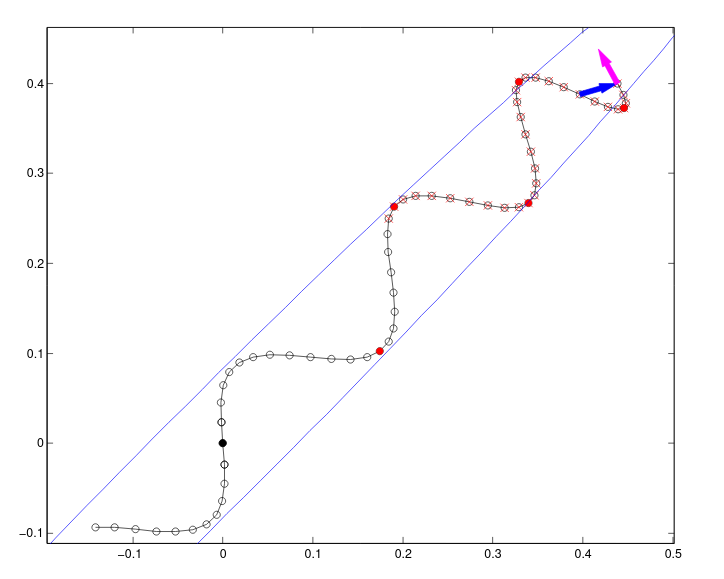
\includegraphics[width=\linewidth]{Screenshot_2020-07-13 Hoffman_Gelman_NUTS pdf.png}
%     % \caption{Caption}
%     % \label{fig:my_label}
% \end{figure}
% \footnotesize
% Figure has been copied from Hoffman \& Gelman (2014) \cite{hoffman2014no}

% \end{column}
% \end{columns}
% \end{frame}

\begin{frame}{NUTS}
\begin{columns}
\begin{column}{0.5\textwidth}
    \begin{itemize}
        \item \textbf{Metropolis-Hastings}
        \begin{itemize}
            \item \color<.>{black} Convergence takes long due to inefficient pathways
        \end{itemize}
        \color{gray}
        \item Hamiltonian Monte Carlo
        \item NUTS
    \end{itemize}
\end{column}
\begin{column}{0.5\textwidth}
\begin{figure}
    \centering
    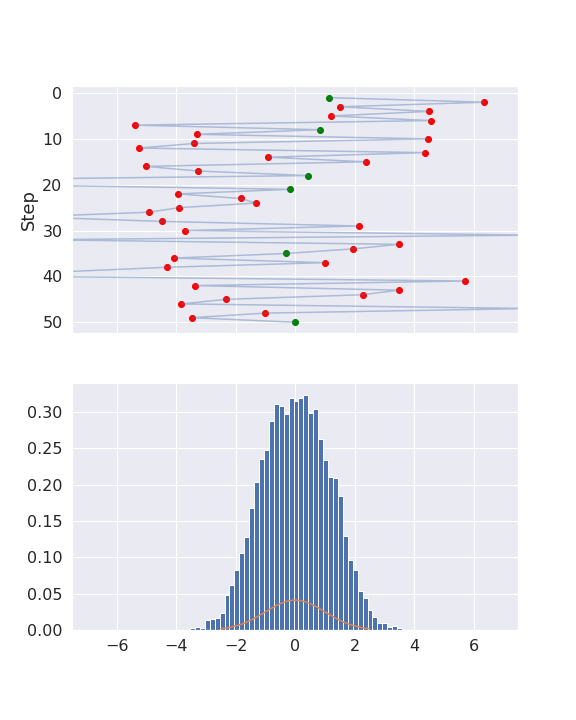
\includegraphics[width=\linewidth]{samplingresult.png}
    % \caption{Caption}
    % \label{fig:my_label}
\end{figure}

\end{column}
\end{columns}
\end{frame}

\begin{frame}{NUTS}
\begin{columns}
\begin{column}{0.5\textwidth}
    \begin{itemize}
    \color{gray}
        \item Metropolis-Hastings
        \color{black}
        \item \textbf{Hamiltonian Monte Carlo}
        \begin{itemize}
            \item Faster convergence
            \item Need to pick values for path-length $L$ and step-size $\epsilon$
        \end{itemize}
        \color{gray}
        \item NUTS
    \end{itemize}
\end{column}
\begin{column}{0.5\textwidth}
\begin{figure}
    \centering
    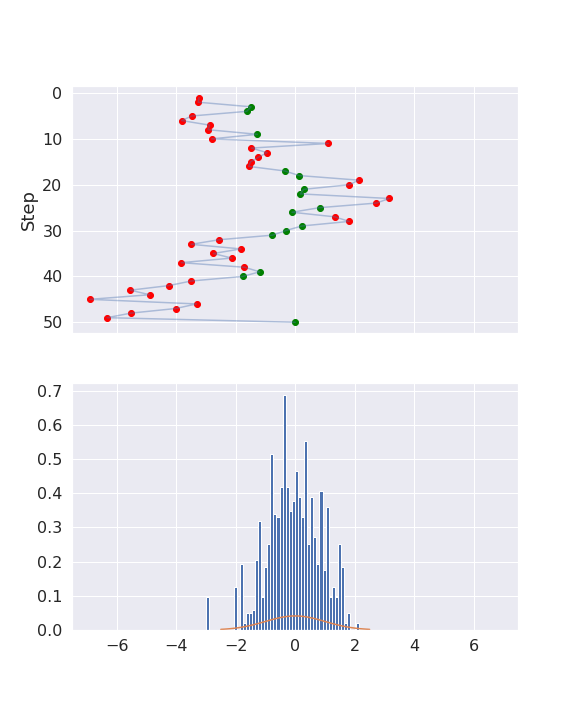
\includegraphics[width=\linewidth]{samplingresult_hmc.png}
    % \caption{Caption}
    % \label{fig:my_label}
\end{figure}

\end{column}
\end{columns}
\end{frame}


\begin{frame}{NUTS}
\begin{columns}
\begin{column}{0.5\textwidth}
    \begin{itemize}
    \color{gray}
        \item Metropolis-Hastings
        \item Hamiltonian Monte Carlo
        \color{black}
        \item \textbf{NUTS}
        \begin{itemize}
            \item Automatically tunes path-length $L$ and step-size $\epsilon$
        \end{itemize}
    \end{itemize}
\end{column}
\begin{column}{0.5\textwidth}
\begin{figure}
    \centering
    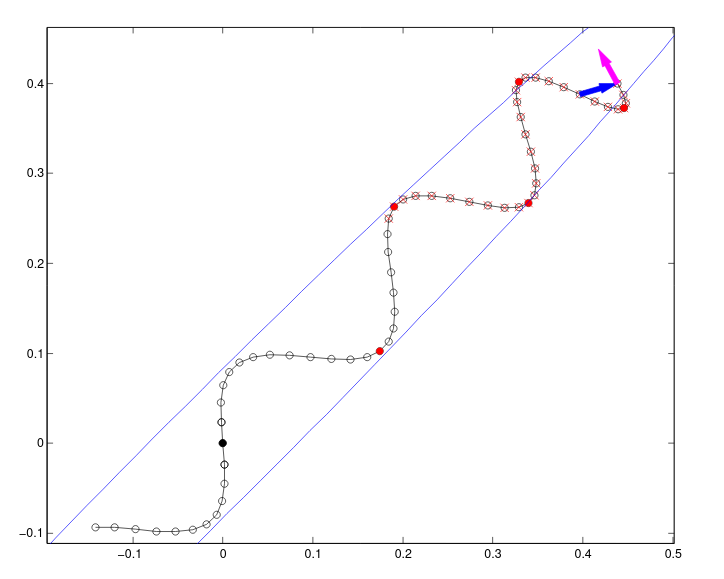
\includegraphics[width=\linewidth]{Screenshot_2020-07-13 Hoffman_Gelman_NUTS pdf.png}
    % \caption{Caption}
    % \label{fig:my_label}
\end{figure}
\footnotesize
Figure has been copied from Hoffman \& Gelman (2014) \cite{hoffman2014no}

\end{column}
\end{columns}
\end{frame}


\begin{frame}{ADVI}
\begin{columns}
\begin{column}{0.6\textwidth}
\begin{itemize}
    \item Variational inference
    \begin{itemize}
        \item Approach $P(\theta|\bm{X})$ by initializing $Q(\zeta)$ and minimize $D_{KL}(Q||P)$
        %$D_{KL}(Q||P) = \int q(\bm{\theta}) \log{\frac{q(\bm{\theta})}{p(\bm{\theta}|\bm{x})}}$
        \item $D_{KL}(Q||P) = \text{evidence} - \text{ELBO}$
        \item $\text{Evidence}$ is independent of $Q$
        % \item $D_{KL}(Q||P)$ is non-negative
        
    \end{itemize}
    \item ADVI automatizes this process
\end{itemize}
\end{column}
\begin{column}{0.4\textwidth}
\begin{figure}
    \centering
    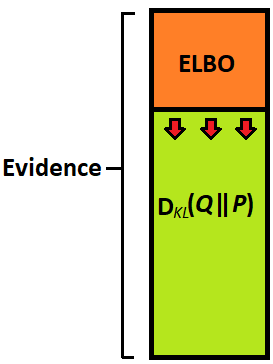
\includegraphics[width=\linewidth]{ELBO.png}
    % \caption{Caption}
    % \label{fig:my_label}
\end{figure}
\end{column}
\end{columns}
\end{frame}



% \begin{frame}
% \frametitle{Model}
% % diagram of pseudocode
% \begin{itemize}
%     \item Initiate PPCA
%     \item Visualize latent space
%     \item Guess number of clusters using data in latent space
%     \item Perform MoPPCAs with estimated number of clusters
%     \item For each found cluster in latent space, estimate number of clusters and perform MoPPCAs
%     \item Repeat until maximum number of levels is reached or until no more sub-clusters are found
% \end{itemize}

% \end{frame}
% \subsection{Automatic clustering}


\section{Methods}

\subsection{Data}

\begin{frame}
\frametitle{Data}
\begin{itemize}
    \item Simulated
    \begin{itemize}
        % \item 5 simple Splatter data-sets: 500 cells, 5/25/50/150/250 genes and 5 cell types
        % \item 5 complex Splatter data-sets: 750 cells, 5/25/50/150/250 genes and 6 cell types
        \item 10 Splatter data-sets varying in complexity and number of genes 
        \item 5 - 250 genes
    \end{itemize}
    \item Experimental
    \begin{itemize}
        \item Darmanis \textit{et al.} \cite{darmanis2015survey}
        % : 22088 genes, 466 data-points, 10 cell types
        \item Nestorowa \textit{et al.} \cite{nestorowa2016single}
        % : 4774 genes, 1656 data-points, 3 cell types
        \item Both were filtered to include only 500 genes with largest variance
    \end{itemize}
\end{itemize}
\end{frame}

\subsection{Experiment set-up}

\begin{frame}
\frametitle{Experiment set-up}
\begin{itemize}
    \item HmPPCAs was compared with PPCA, t-SNE and UMAP
    \item Visualization performance was scored on cell type separability
    \begin{itemize}
        \item Multinomial logistic regression on latent data-sets using 5-fold cross-validation
    \end{itemize}
    % \item One accuracy score was obtained for every plot.
    % \begin{itemize}
    %     \item Since HmPPCAs produces multiple plots, accuracy was average over every level within model
    %     \item Level with highest accuracy is reported
    % \end{itemize}
\end{itemize}

\begin{figure}
\begin{subfigure}{.4\textwidth}
    \centering
    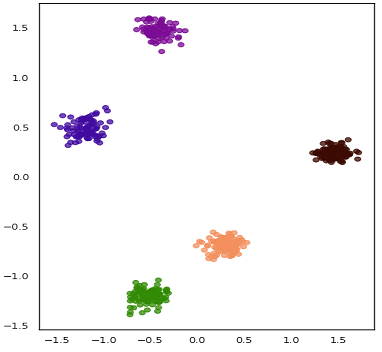
\includegraphics[width=.8\linewidth]{easy.png}
    \caption{\footnotesize Well separated, easy to predict cell type of new data-points}
\end{subfigure}
\begin{subfigure}{.4\textwidth}
    \centering
    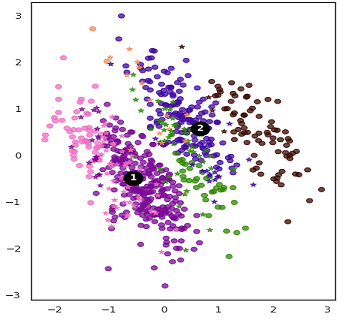
\includegraphics[width=.8\linewidth]{difficult.png}
    \caption{\footnotesize Badly separated, difficult to predict cell type of new data-points}
\end{subfigure}
\end{figure}

\end{frame}

\section{Results}

% \begin{frame}
% \frametitle{Results - accuracy}
% % \begin{itemize}
% %     \item Results Splatter data-sets
% %     \item Result Darmanis
% %     \item Result Nestorowa
% % \end{itemize}

% % \begin{table}
% % \setlength{\tabcolsep}{3pt}
% % \caption{\tiny \textbf{Accuracy of multinomial logistic regressions on the latent data-sets found by each model in a $5$-fold cross-validation scheme}}
% %     \label{tab:results}
% %     \centering
% % \tiny
% % \begin{tabular}{l|rrrrr|rrrrr|r|r}
% %       & \multicolumn{5}{r}{Splatter simple} & \multicolumn{5}{r}{Splatter complex} & Darmanis & Nestorowa \\
% %       genes & 5 & 25 & 50 & 150 & 250 & 5 & 25 & 50 & 150 & 250 & 500 & 500 \\
% %       \hline
    
% %     \makecell{PPCA\\(NUTS)} & \textbf{1.00} & 0.88 & 0.99 & 0.97 & 0.94 &
% %     0.80 & 0.68 & 0.82 & 0.81 & 0.77 & 0.60 & 0.73\\
    
% %     \makecell{HmPPCAs\\(NUTS)} & \textbf{1.00} & \textbf{1.00} & \textbf{1.00} & 0.97 & \textbf{1.00} &
% %     0.90 & 0.82 & 0.89 & 0.82 & 0.69 & 0.70 & 0.79\\
    
% %     \makecell{PPCA\\(VB)} & \textbf{1.00} & 0.88 & 0.99 & 0.96 & 0.94 &
% %     0.80 & 0.69 & 0.81 & 0.82 & 0.76 & 0.73 & 0.73\\
    
% %     \makecell{HmPPCAs\\(VB)} & \textbf{1.00} & \textbf{1.00} & \textbf{1.00} & 0.98 & \textbf{1.00} &
% %     0.90 & 0.91 & 0.90 & 0.94 & 0.79 & 0.73 & 0.79\\
    
% %     UMAP & \textbf{1.00} & \textbf{1.00} & \textbf{1.00} & \textbf{1.00} & \textbf{1.00} &
% %     0.95 & \textbf{0.98} & 0.98 & \textbf{1.00} & \textbf{1.00} & \textbf{0.82} & \textbf{0.82}\\
    
% %     t-SNE & \textbf{1.00} & \textbf{1.00} & \textbf{1.00} & \textbf{1.00} & \textbf{1.00} & 
% %     \textbf{0.95} & 0.94 & \textbf{1.00} & \textbf{1.00} & \textbf{1.00} & 0.76 & 0.80\\
% % \end{tabular}
% % \end{table}

% \begin{figure}
%     \centering
%     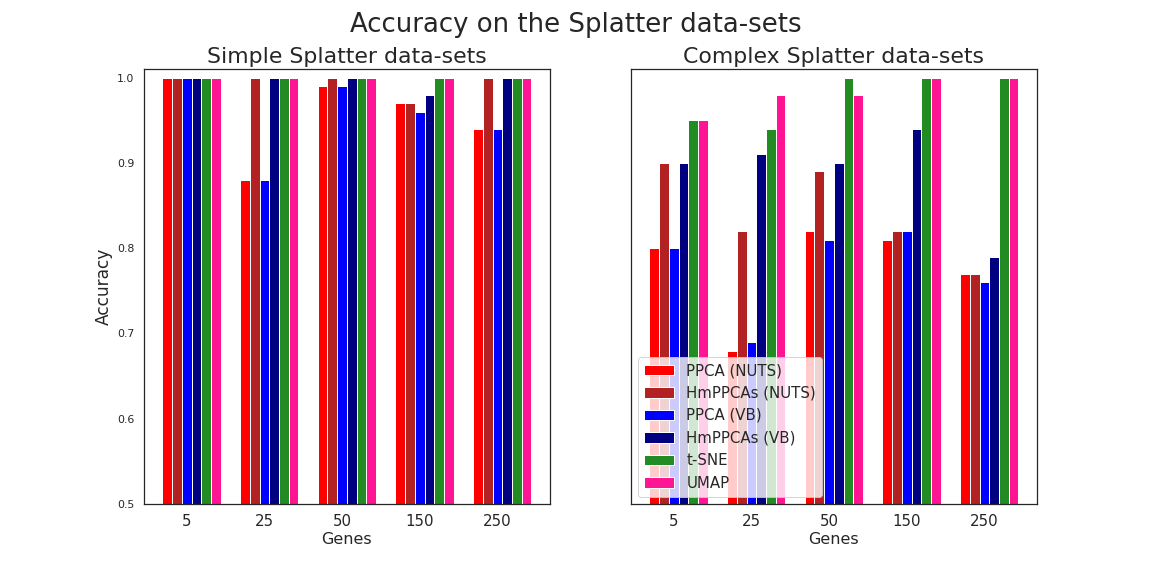
\includegraphics[width=\linewidth]{Splatter_Accuracy_all.png}
%     % \caption{Accuracy on Splatter data-sets}
%     % \label{fig:my_label}
% \end{figure}

% \end{frame}

% \begin{frame}{Results - accuracy}
%     \begin{figure}
%         \centering
%         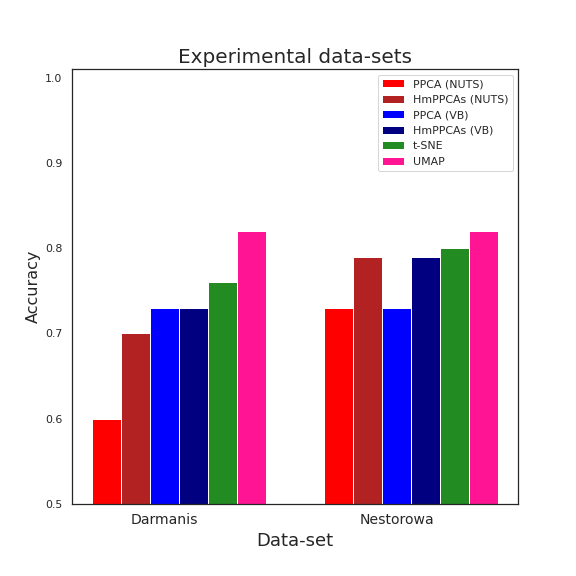
\includegraphics[width=0.6\linewidth]{Splatter_Accuracy_exp.png}
%         % \caption{Caption}
%         % \label{fig:my_label}
%     \end{figure}
% \end{frame}

\begin{frame}{Example of HmPPCAs on a Splatter data-set}
    \begin{figure}
        \centering
        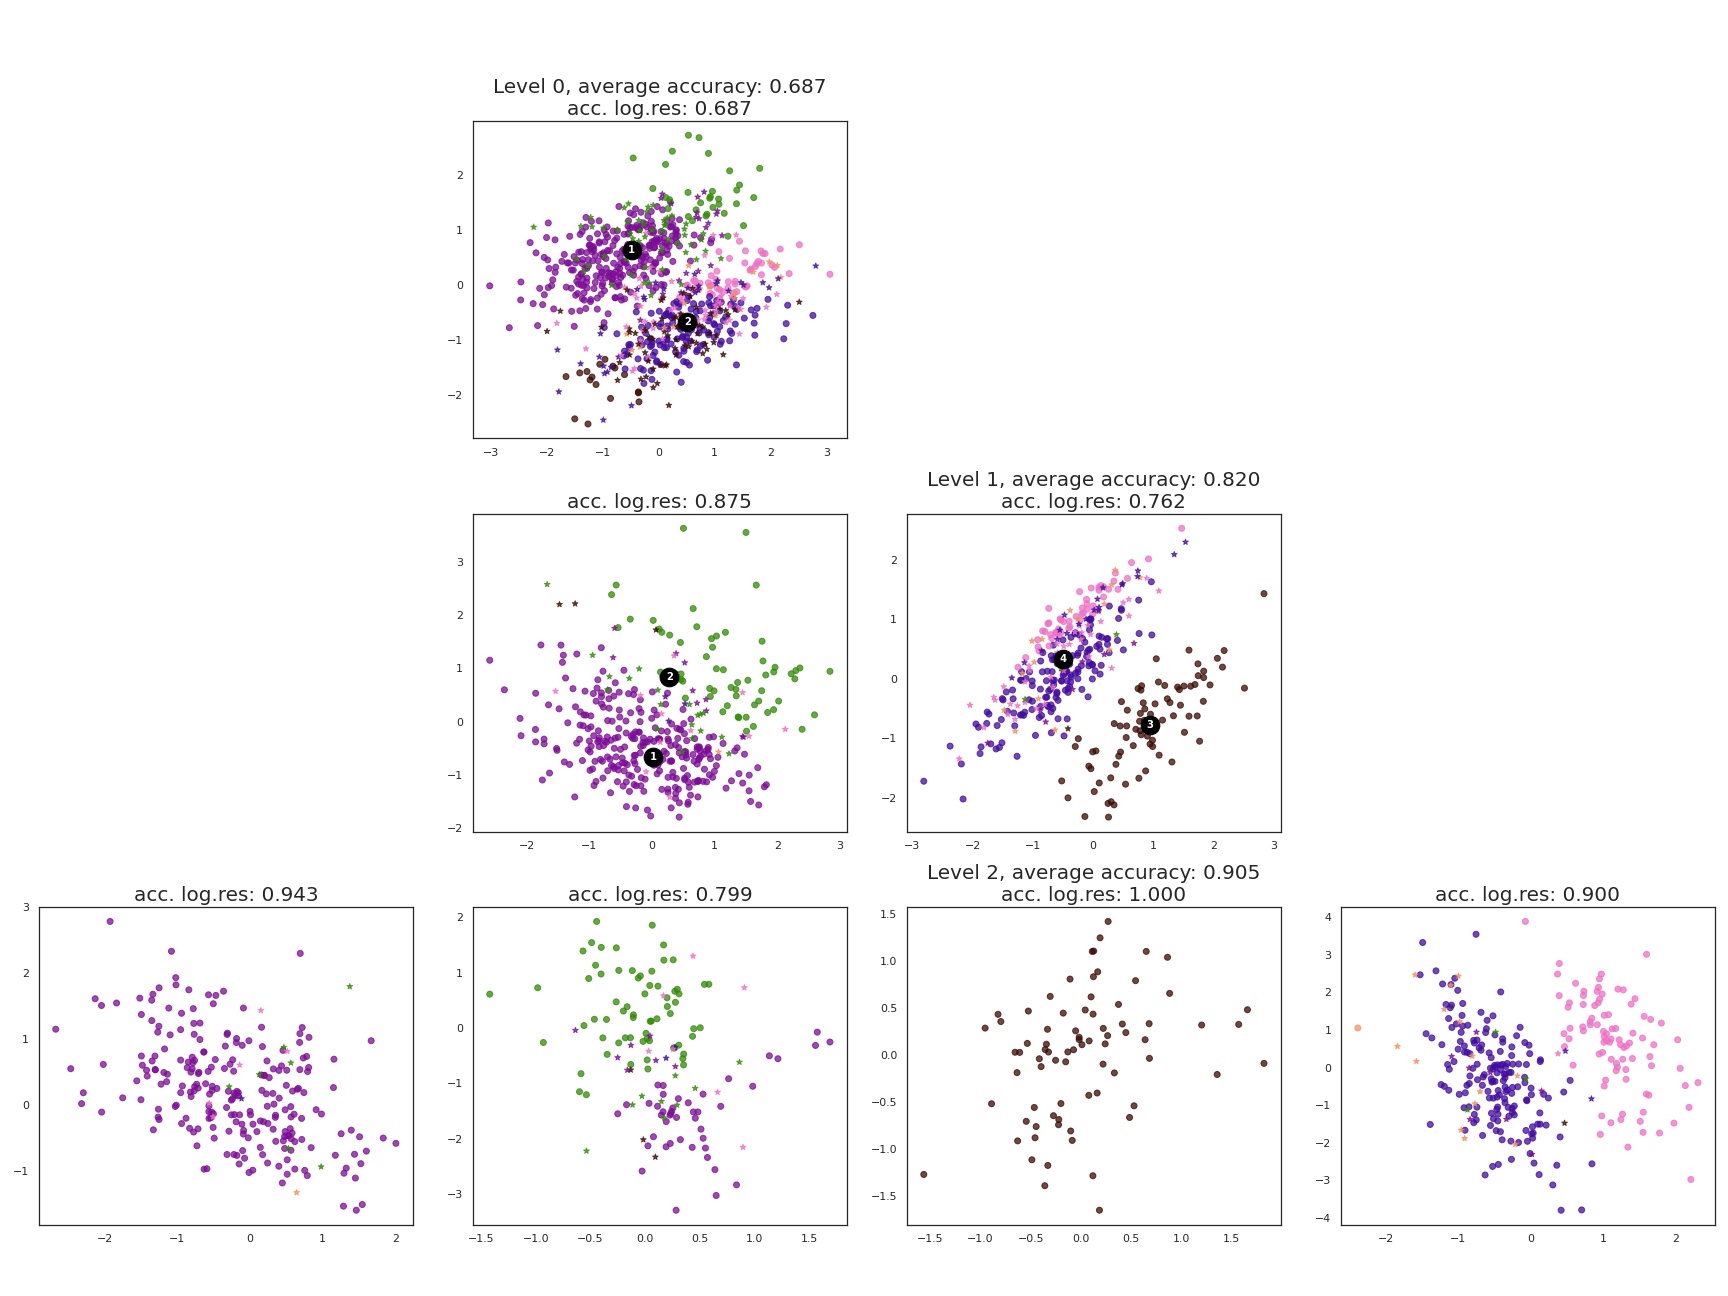
\includegraphics[width=.8\linewidth]{complex_25_vb.png}
        % \caption{Caption}
        % \label{fig:my_label}
    \end{figure}
\end{frame}

\begin{frame}{Results}
% \begin{columns}
% \begin{column}{0.5\linewidth}
\begin{itemize}
    \item HmPPCAs almost always scored higher than PPCA
    \item t-SNE and UMAP consistently outperformed HmPPCAs
\end{itemize}
% \end{column}
% \begin{column}{0.5\linewidth}
% \begin{figure}
%     \centering
%     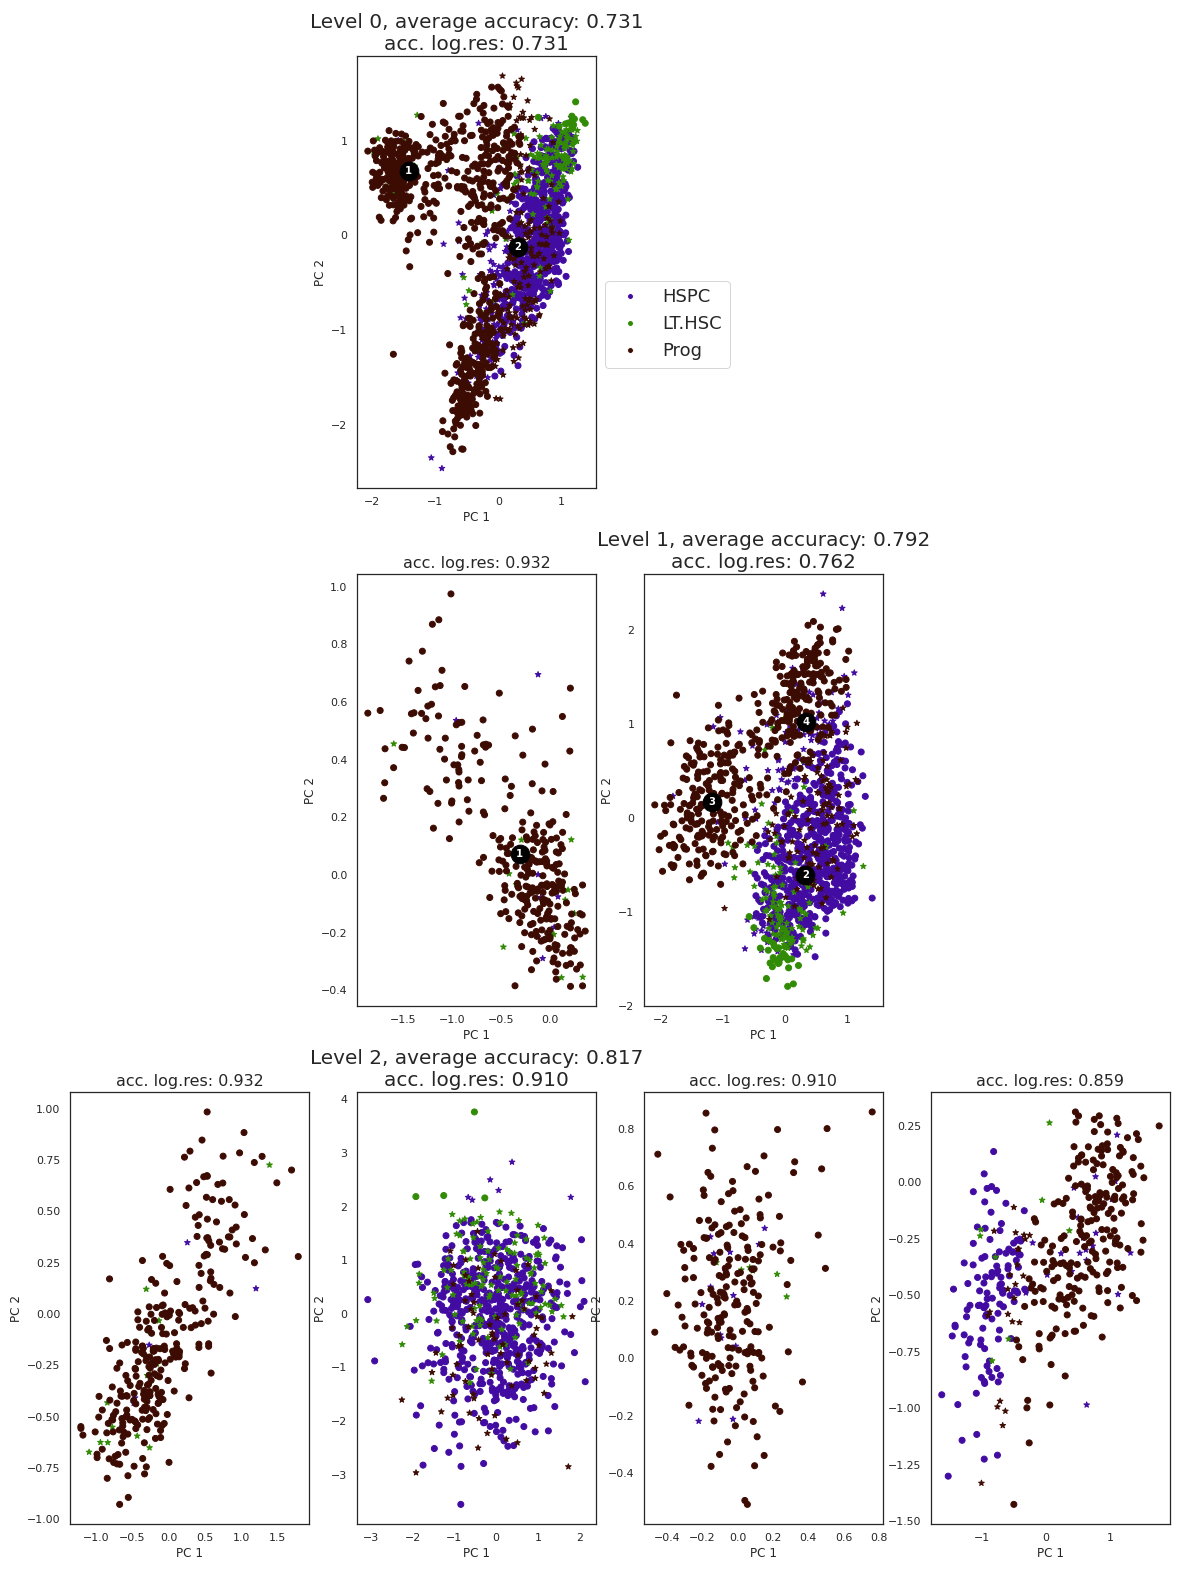
\includegraphics[width=.9\linewidth]{Nestorowa_tree_NUTS.png}
%     % \caption{Caption}
%     % \label{fig:my_label}
% \end{figure}
% \end{column}
% \end{columns}
\end{frame}


% \begin{frame}{Results - computation time}
% \centering
% Computation time of Simple Splatter data-sets
    
% \begin{figure}[h]
% \centering
% \begin{subfigure}{.5\textwidth}
%   \centering
%   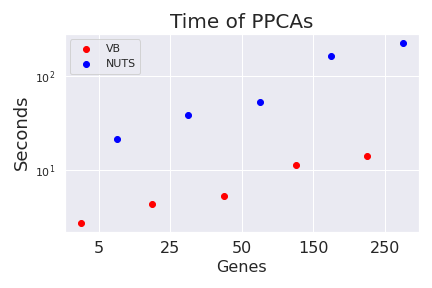
\includegraphics[width=\linewidth]{time_ppca_small.png}
% \end{subfigure}%
% \begin{subfigure}{.5\textwidth}
%   \centering
%   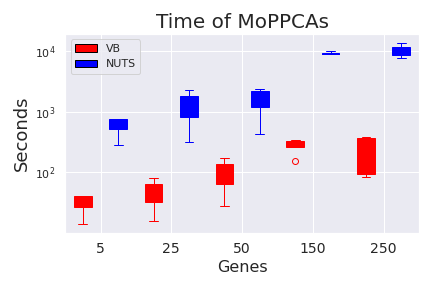
\includegraphics[width=\linewidth]{time_moppcas_small.png}
% \end{subfigure}
% \small
% % \caption{\textbf{t-SNE and UMAP performance on the Splatter data-sets.}}
% \end{figure}
    
% \end{frame}

% \begin{frame}{Results - computation time}
% \centering
% Computation time of Complex Splatter data-sets
    
% \begin{figure}[h]
% \centering
% \begin{subfigure}{.5\textwidth}
%   \centering
%   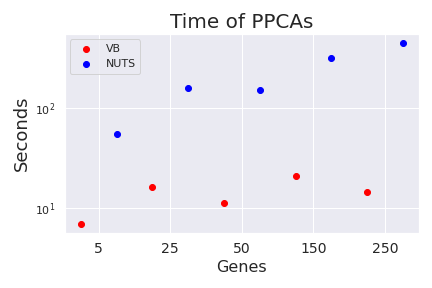
\includegraphics[width=\linewidth]{time_ppca_big.png}
% \end{subfigure}%
% \begin{subfigure}{.5\textwidth}
%   \centering
%   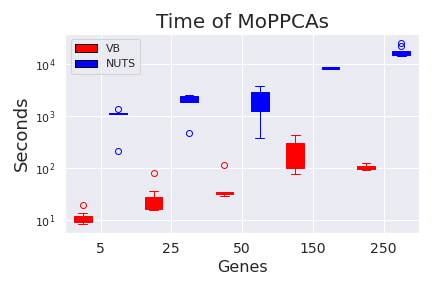
\includegraphics[width=\linewidth]{time_moppcas_big.png}
% \end{subfigure}
% \small
% % \caption{\textbf{t-SNE and UMAP performance on the Splatter data-sets.}}
% \end{figure}
    
% \end{frame}

\section{Conclusions}

\begin{frame}
\frametitle{Conclusions}
\begin{itemize}
    \item HmPPCAs not as accurate as UMAP or t-SNE
    \item Adding hierarchy did improve on a standard PPCA
    \item HmPPCAs outperfomed UMAP and t-SNE in earlier literature
    % \item Might be due to:
    \begin{itemize}
        \item Errors in automatic clustering
        \item Incorrect initialization MoPPCAs
        % prior/initialization/constraints on $\sigma^2$
    \end{itemize}
    \item Easy to incorporate more elements in the model due to probabilistic programming (e.g. zero-inflation)
    % \item ADVI and NUTS perform equally well, but ADVI is much faster
\end{itemize}
\end{frame}

\appendix

\begin{frame}[shrink=20]

\frametitle{Thank you!}
\textbf{References:}
\footnotesize
\bibliographystyle{unsrtnat} % Use the "unsrtnat" BibTeX style for formatting the Bibliography

\bibliography{refs}


\end{frame}


\begin{frame}

\begin{figure}
    \centering
    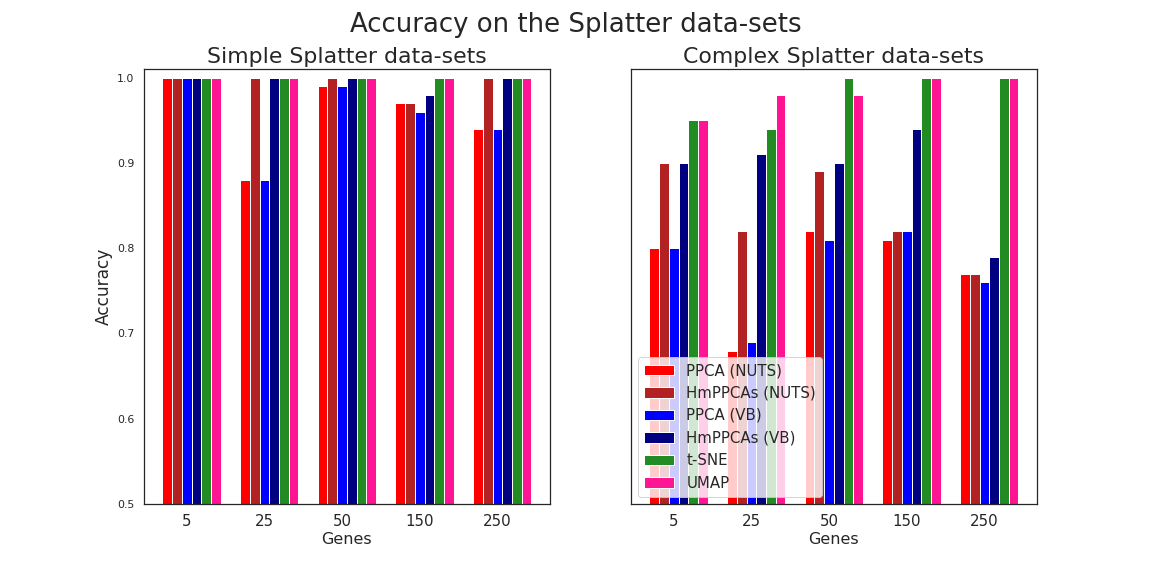
\includegraphics[width=\linewidth]{Splatter_Accuracy_all.png}
    % \caption{Accuracy on Splatter data-sets}
    % \label{fig:my_label}
\end{figure}

\end{frame}

\begin{frame}{Results - accuracy}
    \begin{figure}
        \centering
        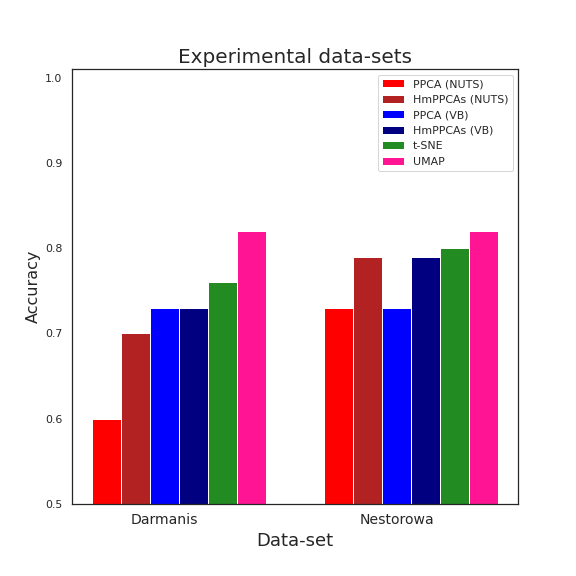
\includegraphics[width=0.6\linewidth]{Splatter_Accuracy_exp.png}
        % \caption{Caption}
        % \label{fig:my_label}
    \end{figure}
\end{frame}

\begin{frame}
\frametitle{Results - accuracy}
% \begin{itemize}
%     \item Results Splatter data-sets
%     \item Result Darmanis
%     \item Result Nestorowa
% \end{itemize}

\begin{table}
\setlength{\tabcolsep}{3pt}
\caption{\tiny \textbf{Accuracy of multinomial logistic regressions on the latent data-sets found by each model in a $5$-fold cross-validation scheme}}
    \label{tab:results}
    \centering
\tiny
\begin{tabular}{l|rrrrr|rrrrr|r|r}
      & \multicolumn{5}{r}{Splatter simple} & \multicolumn{5}{r}{Splatter complex} & Darmanis & Nestorowa \\
      genes & 5 & 25 & 50 & 150 & 250 & 5 & 25 & 50 & 150 & 250 & 500 & 500 \\
      \hline
    
    \makecell{PPCA\\(NUTS)} & \textbf{1.00} & 0.88 & 0.99 & 0.97 & 0.94 &
    0.80 & 0.68 & 0.82 & 0.81 & 0.77 & 0.60 & 0.73\\
    
    \makecell{HmPPCAs\\(NUTS)} & \textbf{1.00} & \textbf{1.00} & \textbf{1.00} & 0.97 & \textbf{1.00} &
    0.90 & 0.82 & 0.89 & 0.82 & 0.69 & 0.70 & 0.79\\
    
    \makecell{PPCA\\(VB)} & \textbf{1.00} & 0.88 & 0.99 & 0.96 & 0.94 &
    0.80 & 0.69 & 0.81 & 0.82 & 0.76 & 0.73 & 0.73\\
    
    \makecell{HmPPCAs\\(VB)} & \textbf{1.00} & \textbf{1.00} & \textbf{1.00} & 0.98 & \textbf{1.00} &
    0.90 & 0.91 & 0.90 & 0.94 & 0.79 & 0.73 & 0.79\\
    
    UMAP & \textbf{1.00} & \textbf{1.00} & \textbf{1.00} & \textbf{1.00} & \textbf{1.00} &
    0.95 & \textbf{0.98} & 0.98 & \textbf{1.00} & \textbf{1.00} & \textbf{0.82} & \textbf{0.82}\\
    
    t-SNE & \textbf{1.00} & \textbf{1.00} & \textbf{1.00} & \textbf{1.00} & \textbf{1.00} & 
    \textbf{0.95} & 0.94 & \textbf{1.00} & \textbf{1.00} & \textbf{1.00} & 0.76 & 0.80\\
\end{tabular}
\end{table}

\end{frame}

% \begin{frame}{NUTS}
% \begin{columns}
% \begin{column}{0.5\textwidth}
%     \begin{itemize}
%         \item \textbf{Metropolis-Hastings}
%         \begin{itemize}
%             \item \color<.>{black} Convergence takes long due to inefficient pathways
%         \end{itemize}
%         \color{gray}
%         \item Hamiltonian Monte Carlo
%         \item NUTS
%     \end{itemize}
% \end{column}
% \begin{column}{0.5\textwidth}
% \begin{figure}
%     \centering
%     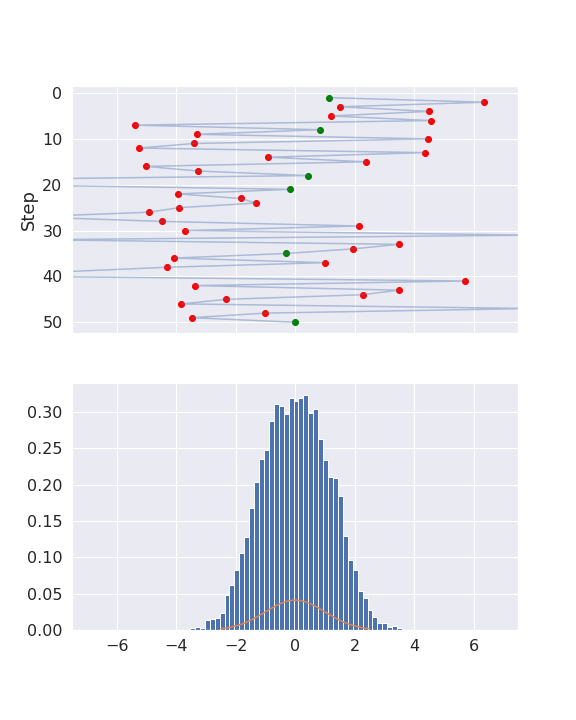
\includegraphics[width=\linewidth]{samplingresult.png}
%     % \caption{Caption}
%     % \label{fig:my_label}
% \end{figure}

% \end{column}
% \end{columns}
% \end{frame}

% \begin{frame}{NUTS}
% \begin{columns}
% \begin{column}{0.5\textwidth}
%     \begin{itemize}
%     \color{gray}
%         \item Metropolis-Hastings
%         \color{black}
%         \item \textbf{Hamiltonian Monte Carlo}
%         \begin{itemize}
%             \item Faster convergence
%             \item Need to pick values for path-length $L$ and step-size $\epsilon$
%         \end{itemize}
%         \color{gray}
%         \item NUTS
%     \end{itemize}
% \end{column}
% \begin{column}{0.5\textwidth}
% \begin{figure}
%     \centering
%     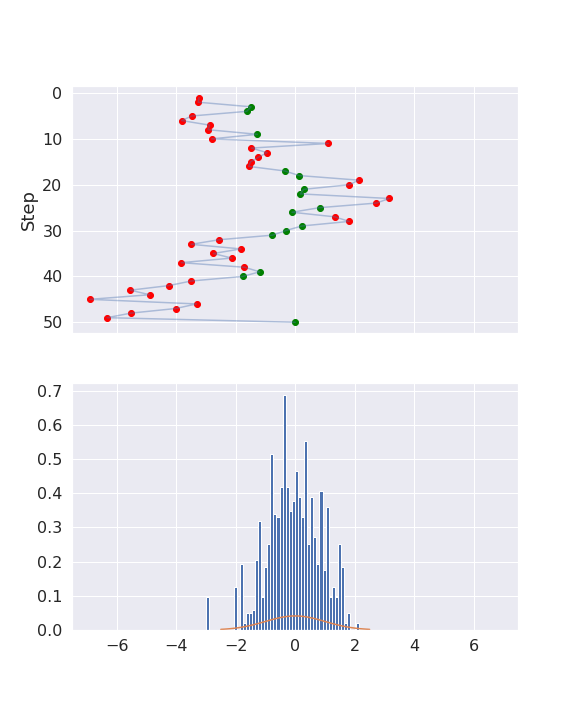
\includegraphics[width=\linewidth]{samplingresult_hmc.png}
%     % \caption{Caption}
%     % \label{fig:my_label}
% \end{figure}

% \end{column}
% \end{columns}
% \end{frame}


% \begin{frame}{NUTS}
% \begin{columns}
% \begin{column}{0.5\textwidth}
%     \begin{itemize}
%     \color{gray}
%         \item Metropolis-Hastings
%         \item Hamiltonian Monte Carlo
%         \color{black}
%         \item \textbf{NUTS}
%         \begin{itemize}
%             \item Automatically tunes path-length $L$ and step-size $\epsilon$
%         \end{itemize}
%     \end{itemize}
% \end{column}
% \begin{column}{0.5\textwidth}
% \begin{figure}
%     \centering
%     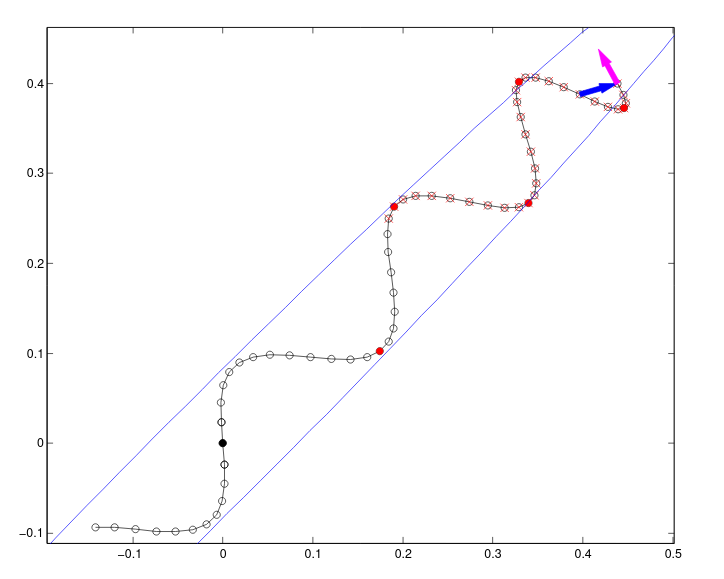
\includegraphics[width=\linewidth]{Screenshot_2020-07-13 Hoffman_Gelman_NUTS pdf.png}
%     % \caption{Caption}
%     % \label{fig:my_label}
% \end{figure}
% \footnotesize
% Figure has been copied from Hoffman \& Gelman (2014) \cite{hoffman2014no}

% \end{column}
% \end{columns}
% \end{frame}

\begin{frame}{Automatic clustering}
    \begin{itemize}
        \item Fit GMM models on latent data, while varying the number of clusters
        \item Compute BIC: $BIC = k \ln{n} - 2 \ln{\mathcal{L}}$, 
        \begin{itemize}
            \item $n$: number of data-points, $k$: number of clusters, $\mathcal{L}$: likelihood of model
        \end{itemize}
        \item Choose model with lowest BIC for the intialization of MoPPCAs
    \end{itemize}
\end{frame}

\end{document}
